\begin{enumerate}[label=\thesection.\arabic*.,ref=\thesection.\theenumi]
\numberwithin{equation}{enumi}
\item The open loop transfer function of a unity feedback system is given by
\begin{align}
\label{eq:ee18btech11007_system}
 G(s)=\frac{\pi e^{-0.25s}}{s}
\end{align}
\item Find $\text{Re} \cbrak{G(\j \omega)}$ and $\text{Im} \cbrak{G(\j \omega)}$.
\\
\solution From \eqref{eq:ee18btech11007_system},
%
 \begin{align}
G(j\omega)&=-\frac{\pi}{\omega}(\sin{0.25\omega}+j\cos{0.25\omega})
\end{align}
\begin{align}
 \text{Re} \cbrak{G(\j \omega)}=-\frac{\pi}{\omega}(\sin{0.25\omega}) 
\end{align}
\begin{align}
 \text{Im} \cbrak{G(\j \omega)}=-\frac{\pi}{\omega}(j\cos{0.25\omega}) 
\end{align}
%
\item Sketch the Nyquist plot.
\\
\solution The Nyquist plot is a graph of $\text{Re} \cbrak{G(\j \omega)}$  vs $\text{Im} \cbrak{G(\j \omega)}$.
The following python code generates the Nyquist plot in Fig.  \ref{fig:ee18btech11007}
\begin{lstlisting}
codes/ee18btech11007.py
\end{lstlisting}
%
\begin{figure}[!h]
  \includegraphics[width=\columnwidth]{./figs/ee18btech11007.eps}
  \caption{}
  \label{fig:ee18btech11007}
\end{figure}
%
\item Find the point at which the Nyquist plot of G(s) passes through the negative real axis
\\
\solution  Nyquist plot cuts the negative real axis at $\omega $ for which 
\begin{align}
\angle G(\j\omega)=-\pi
\label{eq:ee18btech11007_system_neg_real}
\end{align}
From \eqref{eq:ee18btech11007_system},
\begin{align}
 G(\j\omega)&=\frac{\pi e^{-\frac{\j\omega}{4}}}{\j\omega} = \frac{\pi e^{-\j\brak{\frac{\omega}{4}+\frac{\pi}{2}}}}{\omega}
\\
\implies \angle{ G(\j\omega)} &= -\brak{\frac{\omega}{4}+\frac{\pi}{2}}
\label{eq:ee18btech11007_system_ang}
\end{align}
From \eqref{eq:ee18btech11007_system_ang} and \eqref{eq:ee18btech11007_system_neg_real}, 
\begin{align}
\frac{\omega}{4}+\frac{\pi}{2} &= \pi
\\
\implies \omega = 2\pi
\end{align}
Also, from \eqref{eq:ee18btech11007_system},
\begin{align}
\label{eq:ee18btech11007_system_mod}
\abs{ G(\j\omega)}&=\frac{\pi }{\abs{\omega}}
\\
\implies \abs{ G(\j2\pi)} &= \frac{1}{2}
\end{align}
\begin{table}[!ht]
\centering
\begin{enumerate}[label=\thesection.\arabic*.,ref=\thesection.\theenumi]
\numberwithin{equation}{enumi}

\item Question-The open loop transfer function of a unity feedback system is given by
\begin{align*}
 G(s)=\frac{\pi e^{-0.25s}}{s}
\end{align*}
\item Find  $\text{Re} \cbrak{G(\j \omega)}$ and  $\text{Im} \cbrak{G(\j \omega)}$
\newline
\solution 
substitute \begin{align}
S=j\omega
\end{align}
we get \begin{align}
G(j\omega)&=-\frac{\pi}{\omega}(\sin{0.25\omega}+j\cos{0.25\omega})
\end{align}
\begin{align}
 \text{Re} \cbrak{G(\j \omega)}=-\frac{\pi}{\omega}(\sin{0.25\omega}) 
\end{align}
\begin{align}
 \text{Im} \cbrak{G(\j \omega)}=-\frac{\pi}{\omega}(j\cos{0.25\omega}) 
\end{align}
\item Sketch the Nyquist plot.
\\
\solution The Nyquist plot is a graph of $\text{Re} \cbrak{G(\j \omega)}$  vs $\text{Im} \cbrak{G(\j \omega)}$.
The following python code generates the Nyquist plot in Fig.  \ref{fig:ee18btech11007}
\begin{lstlisting}
codes/ee18btech11007/nyquist.py
\end{lstlisting}
%
\begin{figure}[!h]
  \includegraphics[width=\columnwidth]{./figs/ee18btech11007.eps}
  \caption{}
  \label{fig:ee18btech11007}
\end{figure}
%
\item Find the point at which the Nyquist plot of G(s) passes through negative real axis
\newline
\solution
\begin{align}
G(s)=\frac{\pi e^{-0.25s}}{s}
\end{align}

 Nyquist plot cuts the negative real
Axis at $\omega$ = phase cross over frequency,at phase cross over frequency the phase of nyquist plot becomes -$\pi$ radians.
\
\newline substitute \begin{align}
s=j\omega.\end{align} 
\begin{align}
G(j\omega)&= -\frac{\pi}{\omega}(\sin{0.25\omega}+j\cos{0.25\omega})
\end{align}
\begin{align}
\angle G(j\omega)=-\pi/2 -0.25\omega.
\end{align}
\begin{align}
\angle G(j\omega)|_{\omega=\omega_{pc}}=-\pi
\end{align}
by solving for $\omega$ we get $\omega_{pc}=2\pi$.
\
\newline magnitude at any point is\begin{align}
X=|G(j\omega)|=\frac{\pi}{\omega}.    
\end{align} 
\
\newline substituting $\omega=2\pi$ in magnitude equation we get X=0.5.
\\
\newline so it intersects at (-0.5,0j)
\\
\newline we can verify with the following plot that it intersects at (-0.5,0j)

\\
\item Use Nyquist stability criterion to determine if the system is stable?
\newline
\solution
 \textbf{Nyquist Stability Criterion} - for  the stability of a closed loop transfer function G(s)/(1+G(s)*H(s)) ,the number of poles of G(s)*H(s) on right half of s-plane must equal the number of encirclement of nyquist plot of  G(s)*H(s) about the critical point -1+0j
\\
\newline we must find
\begin{align}
Z=P+N    
\end{align}
\
\begin{tabular}{ |p{4cm}||p{4cm}|  }
 \hline
 
 \hline
 Variable&Description\\
 \hline
 Z&no of poles of G(s)/(1+G(s)*H(s)) in the right half of s-plane\\
 \hline
 P&no of poles of G(s)*H(s) in right half of s-plane \\
 \hline
 N&no of encirclement of nyquist plot of G(s)*H(s) about -1+j0 in clockwise direction\\
 
 \hline
\end{tabular}
\\
\newline NOTE-
\begin{itemize}
\item If a clockwise contour does not encircle zeros nor poles, then the plot will not encircle the origin.
\item If a clockwise contour encircles a zero, then the plot will encircle the origin clockwise once.
\item If a clockwise contour encircles a pole, then the plot will encircle the origin counterclockwise once.
\item clockwise encirclement of nyquist plot is taken as positive and  counterclockwise encirclement of nyquist plot is taken as negative
\end{itemize}
\\
\newline from plot we get N=0 because there are no encirclements about -1+0j,and we already know P=0 since our G(s) doesnt have any poles on right half of s-plane
\begin{align}
Z=0+0=0
\end{align}
$\therefore$ the system is stable.



\end{enumerate}

\caption{}
\label{table:ee18btech11007}
\end{table}
%

\item Find the value of $N$ defined in Table \ref{table:ee18btech11007} from Fig.  \ref{fig:ee18btech11007}.
%
\\
\solution $N = 0$. as there are no encirclements of the nyquist plot of G(s) about -1+0j
\item Find the value of $P$ defined in Table \ref{table:ee18btech11007} from  \eqref{eq:ee18btech11007_system}
\\
\solution $\because H(s) = 1$, $G(s)H(s) = G(s)$. Also, $G(s)$ has a pole at $s = 0$, hence $P = 0$.
\item Use the Nyquist Stability criterion to determine if the system in \ref{eq:ee18btech11007_system} is stable.
\\
\solution \textbf{Nyquist criterion}-the no of encirclements of nyquist plot around origin equals difference of no of zeros and no of poles in the right half of splane, the system is stable if
\begin{align}
\label{eq:ee18btech11007_system_nyquist}
Z = P+N = 0,    
\end{align}
%
where $Z$ is defined in Table \ref{table:ee18btech11007}.   
$\because Z = 0$ from \ref{eq:ee18btech11007_system_nyquist}
,  so the system is stable.
%


\end{enumerate}
